\documentclass[tikz, border=3.14mm]{standalone}
\usepackage{pgfplots}
\pgfplotsset{compat=1.18}
\usepgfplotslibrary{groupplots}

\begin{document}
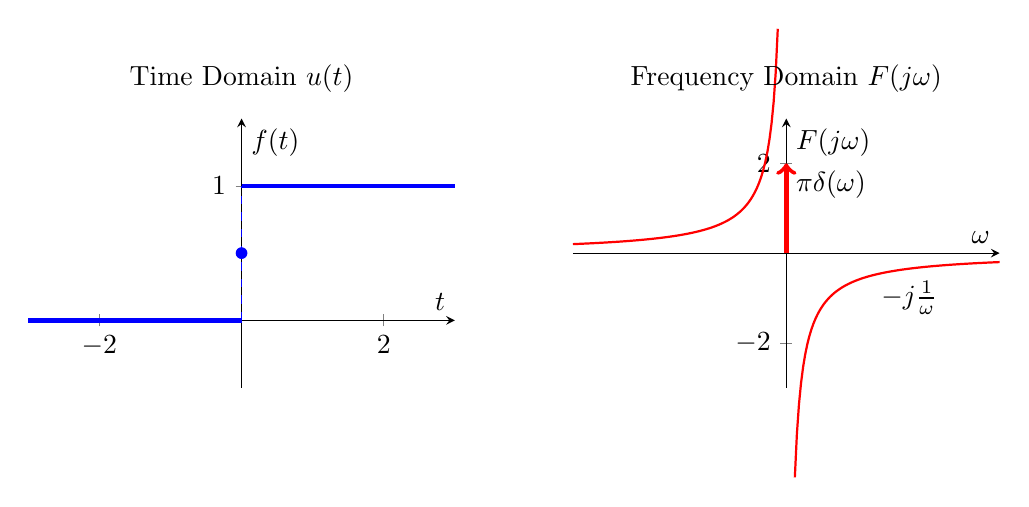
\begin{tikzpicture}
    \begin{groupplot}[
        group style={group size=2 by 1, horizontal sep=1.5cm},
        axis lines = middle,
        width = 7cm, height = 5cm,
        ymin = -0.5, ymax = 1.5,
        grid=none,
        xlabel = {$t$},
        ylabel = {$f(t)$}
    ]
        % Time Domain Unit Step
        \nextgroupplot[
            title = {Time Domain $u(t)$},
            xmin = -3, xmax = 3,
            ytick = {1}
        ]
        \draw[ultra thick, blue] (-3,0) -- (0,0);
        \draw[ultra thick, blue] (0,1) -- (3,1);
        \draw[blue, dashed] (0,0) -- (0,1);
        \node[circle, fill=blue, inner sep=1.5pt] at (0,0.5) {};

        % Frequency Domain Unit Step
        \nextgroupplot[
            title = {Frequency Domain $F(j\omega)$},
            xlabel = {$\omega$},
            ylabel = {$F(j\omega)$},
            xmin = -5, xmax = 5,
            ymin = -3, ymax = 3,
            xtick = \empty,
            clip = false
        ]
        \addplot[thick, red, domain=-5:-0.2, samples=100] {-1/x};
        \addplot[thick, red, domain=0.2:5, samples=100] {-1/x};
        \draw[->, ultra thick, red] (axis cs:0,0) -- (axis cs:0,2);
        \node[anchor=south west] at (axis cs:0, 1) {$\pi \delta(\omega)$};
        \node[anchor=west] at (axis cs:2, -1) {$-j\frac{1}{\omega}$};

    \end{groupplot}
\end{tikzpicture}
\end{document}
